\documentclass[12pt]{report}
\usepackage{amsmath}
\usepackage{amssymb}
\usepackage{amsthm}
\usepackage{enumitem}
\usepackage{graphicx}
\usepackage{multicol}
\usepackage{siunitx}

\newcommand{\e}[1]{e^{#1}}
\newcommand{\ei}[1]{e^{i\left(#1\right)}}
\newcommand{\E}[1]{\times 10^{#1}}
\newcommand{\tagref}[1]{\tag{\ref{#1}}}

\renewcommand\qedsymbol{TENA}

\begin{document}
\DeclareSIUnit{\amu}{amu}
\DeclareSIUnit{\light}{c}
\DeclareSIUnit{\lightyear}{c\cdot yr}
\DeclareSIUnit{\year}{yr}
\DeclareSIUnit{\yr}{yr}

\footnotesize
\chapter*{Practice Problems}
Equations used:
\begin{multicols}{2}
    Vibrational states in molecules:
    \begin{equation*}
        E_N = (N + \frac{1}{2})\hbar \omega; 
        \omega = \sqrt{\frac{k}{m}} = 2\pi f
    \end{equation*}
    Use harmonic mean for mass
    \begin{equation*}
        m = \left( \sum \frac{1}{m_i} \right)^{-1} \left[ = \frac{m_1 \cdot m_2}{m_1 + m_2} \right]
    \end{equation*}
    Rotational energy also exists, from Q.N. $L$
    \begin{equation*}
        E_L = \frac{L(L+1)\hbar^2}{2mR_{eq}^2}
    \end{equation*}

    For dilute gas, go straight to Maxwell-Boltzmann.
    \begin{gather*}
        k = 1.38\E{-23}\,\unit{\joule/\kelvin} = 8.617\E{-5}\,\unit{\eV/\kelvin}\\
        K_{avg} = \frac{3}{2}kT;
        N(E) = \frac{2N}{\sqrt{\pi}(kT)^{3/2}}E^{\frac{1}{2}}\e{-\frac{E}{kT}}
    \end{gather*}

    Approximate tiny distribution integrals.
    \begin{equation*}
        \int_{E_m}^{E_m + \Delta E} N(E) dE \approx N(E) * \Delta E
    \end{equation*}

    \underline{Relativity}
        $\Delta t_0$ is proper time; $L_0$ = proper length
        \begin{gather*}
            \Delta t = \frac{\Delta t_0}{\sqrt{1 - u^2/c^2}}; 
            L = L_0\sqrt{1 - u^2/c^2}\\
            v = \frac{v' - u}{1 + v'u/c^2}; 
            f' = f\sqrt{\frac{1 - u/c}{1 + u/c}}
        \end{gather*}
        Lorentz Transforms
        \footnotesize
        \begin{gather*}
            x' = \frac{x - ut}{\sqrt{1 - u^2/c^2}};
            \begin{matrix}
                y' = y;\\
                z' = z;
            \end{matrix}
            t' = \frac{t - (u/c^2)x}{\sqrt{1 - u^2/c^2}}\\
            v'_x = \frac{v_x - u}{1 - v_x u/c^2};
            v'_y = \frac{v_y \sqrt{1 - u^2 / c^2}}{1 - v_x u/c^2}
            v'_z = \frac{v_z \sqrt{1 - u^2 / c^2}}{1 - v_x u/c^2}
        \end{gather*}
        \normalsize

        Relativity alters momentum and energy

\end{multicols}

\pagebreak
\section*{Problem 1}
    What atoms have the ground state configurations: (a) $1s^2 2s^2 2p^1$, (b)  $1s^2 2s^2 2p^6 3s^1$, (c) $[Ne]3s^2 3p^5$

    \subsection*{Solution}
    \begin{enumerate}[label=(\alph*)]
        \item   Boron (B)
        \item   Sodium (Na)
        \item   Chlorine (Cl)
    \end{enumerate}

\section*{Problem 2}
    What is the ground state configuration of the ion $K^+$?

    \subsection*{Solution}
        \boxed{1s^2 2s^2 2p^6 3s^2 3p^6}

\section*{Problem 3}
    What is the ground state configuration of the ion $S^{-2}$?

    \subsection*{Solution}
        \boxed{1s^2 2s^2 2p^6 3s^2 3p^6}

\section*{Problem 4}
    What is the electron configuration of the first excited state of He?

    \subsection*{Solution}
        \boxed{1s^1 2s^1}
    \pagebreak

\section*{Problem 5}
    For the hydrogen atom in the 3d excited state, give the possible values of $(\ell, m_\ell, s, m_s)$ for the atom.

    \subsection*{Solution}
        $\ell = 2$; $m_\ell \in \{-2, -1, 0, 1, 2\}$; $s = \frac{1}{2}$; $m_s \in \left\{ \frac{1}{2}, -\frac{1}{2} \right\}$

\section*{Problem 6}
    List the quantum numbers $(n, \ell, m_\ell, m_s)$ for all the electrons in a ground state nitrogen atom.

    \subsection*{Solution}
        \begin{tabular}{c | c c c}
            1s & $(1, 0, 0, -\frac{1}{2})$ & $(1, 0, 0, \frac{1}{2})$ &\\
            2s & $(2, 0, 0, -\frac{1}{2})$ & $(2, 0, 0, \frac{1}{2})$ &\\
            2p & $(2, 1, -1, \frac{1}{2})$ & $(2, 1, 0, \frac{1}{2})$ & $(2, 1, 1, \frac{1}{2})$
        \end{tabular}

\section*{Problem 7}
    Infrared photons of wavelength 3440 nm are observed in the emission spectrum of molecular HCl. 
    You suspect that this is from excitations of vibrational modes of the molecule as a harmonic oscillator. 
    The mass of H is 1.008 u and the mass of Cl is 34.97 u where the atomic mass unit $u = 1.63\E{-27}\,\unit{\kilo\gram}$. 
    What is the `spring constant' of this ionic bond? % 490 N/m

    \subsection*{Solution}
        Energy of a photon can be computed from wavelength, so let's do that. 
        \begin{align*}
            E   &=  \frac{hc}{\lambda}
                =   \frac{1240\,\unit{\eV\cdot\nano\meter}}{3440\,\unit{\nano\meter}}
                =   0.36\,\unit{\eV} \times \frac{1.602\E{-19}\,\unit{\joule}}{1\,\unit{\eV}}
                =   5.7672\E{-20}\,\unit{\joule}
        \end{align*}

        This is the difference between two vibrational nodes' energies, or equivalent to $\hbar\omega$.
        Since $\omega = \sqrt{\frac{k}{m}}$, we can from here calculate the spring constant $k$.
        Make sure to use the harmonic mean for the mass.
        \begin{align*}
            E   &=  \hbar\omega = \hbar\sqrt{\frac{k}{m}}\\
            m   &=  \frac{m_1 * m_2}{m_1 + m_2}
                =   \frac{34.97 * 1.008}{34.97 + 1.008}
                =   0.9798\\
            k   &=  \frac{E^2 m}{\hbar^2}
                =   \frac{(5.7672\E{-20}\,\unit{\joule})^2(0.9798 \times 1.63\E{-27}\,\unit{\kilo\gram})}{(1.054\E{-34}\,\unit{\joule\cdot\second})^2}
                =   \boxed{478\,\unit{\newton/\meter}}
        \end{align*}
    \pagebreak

\section*{Problem 8}
    Consider the diatomic molecule $H_2$. 
    You can model it as two point masses (each of mass 1.08 u where $1u = 931.5\,\unit{\mega\eV/\light^2}$) with a separation of 0.074 nm. 
    What is the wavelength of the photons emitted when this `quantum rotor' transitions with the lowest possible energy change? 

    \subsection*{Solution}
        The miminum transition would come from transition between $L = 1$ to $L = 0$.
        We can calculate the energy transition here.
        Don't forget that we use the harmonic mean for the mass.
        \begin{align*}
            E   &=  \frac{L(L+1)\hbar^2}{2mR_{eq}^2}
                =   \frac{1(2)(hc)^2}{(2\pi)^2 2mR_{eq}^2 c^2}
                =   \frac{2(1240\,\unit{\eV\cdot\nano\meter})^2}{(2\pi)^2 (931.5\,\unit{\mega\eV}) (0.074\,\unit{\nano\meter})^2}\\
                &=  \frac{2*1.5376\,\unit{\eV}}{4\pi^2 931.5 * 5.476\E{-3}}
                =   \frac{3.0752\,\unit{\eV}}{64.1}
                =   0.048\,\unit{\eV}\\
            \lambda &=  \frac{hc}{E}
                =   \frac{1240\,\unit{\eV\cdot\nano\meter}}{0.048\,\unit{\eV}}
                =   \boxed{81.2\,\unit{\micro\meter}}
        \end{align*}
    \pagebreak

\section*{Problem 9}
    Consider 1 mol of a dilute He gas at temperature 293 K. 
    (a) What is the mean value of the energy, $E_m$, of an atom? 
    (b) What fraction of the atoms has an energy in an interval of 0.01*$E_m$, centered at $E_m$? 

    \subsection*{Solution (a)}
        Use the Maxwell-Boltzmann energy distribution and find the average kinetic energy.
        \begin{align*}
            K_{avg} &=  \frac{3}{2}kT
                =   \frac{3}{2} * 8.617\E{-5}\,\unit{\eV/\kelvin} * 293\,\unit{\kelvin}
                =   \boxed{37.87\E{-3}\,\unit{\eV}}
        \end{align*}

    \subsection*{Solution (b)}
        Recall the Maxwell-Boltzmann distribution.
        \begin{equation*}
            N(E) = \frac{2N}{\sqrt{\pi}(kT)^{3/2}}E^{1/2}\e{E/kT}
        \end{equation*}

        Divide both sides by the number of total particles, which happens to already be in the equation.
        \begin{equation*}
            \frac{N(E)}{N} = \frac{2}{\sqrt{\pi}(kT)^{3/2}}E^{1/2}\e{E/kT}
        \end{equation*}

        Multiply both by $dE$ and take the integral over the span.
        Use the approximation.
        \begin{align*}
            \int_{0.995\,E_m}^{1.005\,E_m}\frac{N(E)}{N}\,dE    &\approx    \frac{2}{\sqrt{\pi}(kT)^{3/2}}E_m^{1/2}\e{E_m/kT} * \Delta E\\
                &=  \frac{2}{\sqrt{\pi}(25.25\E{-3})^{3/2}}(37.87\E{-3})^{3/2}\e{-\frac{37.87\E{-3}}{25.25\E{-3}}} * 0.01\\
                &=  \frac{32.89\E{-6}}{7.11\E{-3}}
                =   0.0046
        \end{align*}

        This means about \boxed{0.46\%} of all atoms are in that range.
    \pagebreak

\section*{Problem 10}
    The speed of light is the fastest speed that any signal can travel. 
    We say that if two events (A and B) in space time can be connected by a signal that travels at or less than the speed of light then these two events can be causally connected. 
    That is, the earlier event can cause the later event and all possible different observer frames will agree on which event was the earlier event. 
    (Effects can not occur before causes)
    
    (a) Show that if A and B are connected by a light signal in a space-time frame where A happens first, then no matter what other frame observes the events, B always happens later than A.

    But if two events can only be connected by a signal that travels faster than light, which is impossible, then the two events cannot be causally connected- and there can be an observer frame that observes the events to happen simultaneously, a different observer frame observes event A to happen first and event B later; and another observer frame to observe that the event B happens first.

    Pick two events A and B that would be connected by a signal that travels at twice the speed of light and pick A to have happened first and list them.

    (b) What is the relative velocity of a frame where observers in that frame would see A and B happen at the same time?
    What are the relative velocities of frames that would see B happen first?

    \subsection*{Solution (a)}
        If event A causes event B by a light signal, then A and B are colinear in a spacetime diagram along a line of slope 1.
        A would also take place before B. 
        \begin{gather*}
            t_B > t_A\\
            0 < t_B - t_A = \Delta t_0
        \end{gather*}

        Suppose for contradiction that in some frame of reference, event B takes place at the same time or before event A.
        \begin{gather*}
            t_B' \leq t_A'\\
            t_B' - t_A' = \Delta t \leq 0
        \end{gather*}

        If we are in a relativistic frame of reference, we are traveling at a specific speed $u$.
        We can apply the Lorentz transformation for the time here.
        \begin{gather*}
            \Delta t = \frac{\Delta t_0}{\sqrt{1 - u^2/c^2}} \leq 0\\
            \Delta t_0 \leq 0\\
            t_B - t_A \leq 0\\
            t_B \leq t_A
        \end{gather*}

        This is a contradiction.
        As such, B always happens after A.

    \subsection*{Solution (b)}
        Suppose that event A and B have $(x,t)$ coordinates $(2\,\unit{\lightyear}, 1\,\unit{\year})$ and $(4\,\unit{\lightyear}, 2\,\unit{\year})$, respectively.
        We can apply the Lorentz transformation here.
        \begin{gather*}
            t' = 0 = \frac{t - (u/c^2)x}{\sqrt{1 - u^2/c^2}}
        \end{gather*}

        For ths to be equal to zero, $t$ must be equal to $(u/c^2)x$.
        \begin{gather*}
            t = (u/c^2)x\\
            u = \frac{t c^2}{x}
        \end{gather*}

        The value of $\frac{x}{t}$ is $2c$ in this instance.
        We can plug this in.
        \begin{align*}
            u = \frac{c^2}{2c} = \frac{c}{2}
        \end{align*}

        If the frame is traveling at a speed of $\frac{c}{2}$, the events would appear to happen at the same time.
        Any faster and event A would appear to happen after event B.
    \pagebreak

\section*{Problem 11}
    Consider two protons headed towards each other with the same speeds. Each proton has mass $m_p = 938.8\,\unit{\mega\eV/\light^2}$. 
    They collide and create a deuteron with mass $m_d = 1875.6\,\unit{\mega\eV/\light^2}$ and a positively charged particle called the 'pion plus'. 
    The pion particle symbol is $\pi^+$ and its mass is $m_\pi = 139.6\,\unit{\mega\eV/\light^2}$. 
    This interaction can be symbolized with $p^+ + p^+ \to \pi^+ + d^+$.

    (a) What is the minimum kinetic energy that each proton must have in order for this to be able to happen? % 69 MeV

    (b) Say that the two protons head into the collision from opposite directions each with 100 MeV of kinetic energy. 
    How much momentum will the pion have after it is created?

    \subsection*{Solution (a)}
        For the minimum necessary velocity for genesis, we assume that upon being created, the two new particles will be completely immobile, so no kinetic energy.
        This means the only energy after creation is their rest energy, which we can calculate.
        \begin{align*}
            E_{net} &=  m_\pi c^2 + m_d c^2
                =   139.6\,\unit{\mega\eV} + 1875.6\,\unit{\mega\eV}
                =   2015.2\,\unit{\mega\eV}
        \end{align*}

        From here, divide it by two and subtract the rest energy of the proton to find the necessary kinetic energy of each photon.
        \begin{align*}
            E_{p^+} &=  \frac{2015.2}{2}\,\unit{\mega\eV}
                =   1007.6\,\unit{\mega\eV}\\
            K   &=  E_{p^+} - E_0
                =   1007.6\,\unit{\mega\eV} - 938.8\,\unit{\mega\eV}
                =   \boxed{68.8\,\unit{\mega\eV}}
        \end{align*}

        % From here, we can use the total energy of the two photons and find the velocity.
        % \begin{gather*}
        %     2015.2\,\unit{\eV} = \frac{mc^2}{\sqrt{1 - v^2 / c^2}}\\
        %     1 - v^2/c^2 = \left( \frac{mc^2}{2015.2\,\unit{\mega\eV}} \right)^2\\
        %     \frac{v^2}{c^2} = 1 - \left( \frac{938.8\,\unit{\mega\eV}}{2015.2\,\unit{\mega\eV}} \right)^2
        %         =   1 - (0.466)^2
        %         =   1 - 0.217
        %         =   0.783\\
        %     v = \boxed{0.885c}
        % \end{gather*}

    \subsection*{Solution (b)}
        The deuterion, if created immobile, will have only its rest energy, which is the rest energy of the two protons that created it.
        This means the 200\,\unit{\mega\eV} of energy (100\,\unit{\eV} from each proton) will all go to the pion.
        \begin{gather*}
            E^2 =   (pc)^2 + (mc^2)^2\\
            \begin{align*}    
                p^2 &=  \left( \frac{E}{c} \right)^2 - (mc)^2
                    =   (200\,\unit{\mega\eV/\light})^2 - (139.6\,\unit{\mega\eV/\light})^2\\
                    &=  40\E{15}\,\unit{\eV^2/\light^2} - 19.488\E{15}\,\unit{\eV^2/\light^2}
                    =   20.512\E{15}\,\unit{\eV^2/\light^2}
            \end{align*}\\
            p   =   \sqrt{20.512\E{15}\,\unit{\eV^2/\light^2}}
                =   \boxed{143\,\unit{\mega\eV/\light}}
        \end{gather*}

\setcounter{chapter}{7}
\chapter{Many Electron Atoms}
Equations used:
\begin{multicols}{2}
    \begin{gather}
        \label{eq:8.1}
        Z_{eff} = q_{\rm nucleus} - q_{\rm screening\,electrons}\\
        \label{eq:8.2}
        E_n = (-13.6\,\unit{\eV})\frac{Z_{eff}^2}{n^2}
    \end{gather}
    For transition energies:
    \begin{gather}
        \label{eq:8.3}
        \Delta E = 13.6\,\unit{\eV}(Z - 1)^2\left( \frac{1}{n_i^2} - \frac{1}{n_f^2} \right)
    \end{gather}
    For electrons in incomplete shells, exists angular ($L$) \& magnetic ($M_L$) Q.N's:
    \begin{gather}
        |L_i| = \hbar\sqrt{l_i(l_i + 1)}\\
        L_{max} = l_1 + l_2; 
        L_{min} = |l_1 - l_2|\\
        L \in [L_{min}, L_{max}] \cap \mathbb{N}\\
        M_L = \sum m_{l,i};
        M_L \in [-L, L] \cap \mathbb{N}
    \end{gather}
    $S$ can be computed same as $M_L$ but with spin quantum number\\
    Hund's rule: $L = M_{L, max}$, $S = M_{S, max}$; maximize total spin\\
    $\Delta L \in \{0, \pm 1\}; \Delta S = 0$\\
    HeNe laser produces photons
    \begin{gather}
        \lambda = 632.8\,\unit{\nano\meter}; E = 1.96\,\unit{\eV}\\
        E_0 = \sqrt{\frac{2I}{c\varepsilon_0}}; I = \frac{P}{A}
    \end{gather} 
\end{multicols}

\pagebreak
\section{Problem 1} % 8.1
(a) List the six possible sets of quantum numbers $(n, l, m_l, m_s)$ of a 2p electron. 
(b) Suppose we have an atom such as carbon, which has two 2p electrons. 
Ignoring the Pauli principle, how many different possible combinations of quantum numbers of the two electrons are there? 
(c) How many of the possible combinations of part (b) are eliminated by applying the Pauli principle? 
(d) Suppose carbon is in an excited state with configuration $2p^1 3p^1$. 
Does the Pauli principle restrict the choice of quantum numbers for the electrons? 
How many different sets of quantum numbers are possible for the two electrons?

\subsection{Solution (a)}
    \begin{tabular}{c c c}
        $(2, 1, -1, -\frac{1}{2})$ & $(2, 1, 0, -\frac{1}{2})$ & $(2, 1, 1, -\frac{1}{2})$\\
        $(2, 1, -1, \frac{1}{2})$ & $(2, 1, 0, \frac{1}{2})$ & $(2, 1, 1, \frac{1}{2})$
    \end{tabular}

\subsection{Solution (b)}
    Take the triangle number of six (for the six configurations).
    \begin{equation}
        T_6 = \frac{n(n+1)}{2}
            =   \frac{6*7}{2}
            =   \boxed{21}
    \end{equation}

\subsection{Solution (c)}
    Only six, since there are six states and Pauli only excludes them when the two states are identical.
    This totals us at 15 states.

\subsection{Solution (d)}
    The Pauli principle still applies, but it would nt be important here. 
    The two have different values for quantum number $n$.
    Furthermore, we would no longer have to account for duplicates, so we can just multiply the number of possible combinations in each shell.
    This gives us $6 * 6 = \boxed{36}$ possible combinations.
\pagebreak

\section{Problem 3}
\begin{enumerate}[label=(\alph*)]
    \item   How many different sets of quantum numbers $(n, l, m_l, m_s)$ are possible for an electron in the 4f level?
    \item   Suppose a certain atom has three electrons in the 4f level. What is the maximum possible value of the total $m_s$ of the three electrons?
    \item   What is the maximum possible total $m_l$ of three 4f electrons?
    \item   Suppose an atom has ten electrons in the 4f level. What is the maximum possible value of the total $m_s$ of the ten 4f electrons?
    \item   What is the maximum possible total $m_l$ of ten 4f electrons?
\end{enumerate}

\subsection{Solution (a)}
    \begin{equation}
        2(2\ell + 1) = 2(2*3 + 1) = 2*7 = \boxed{14}
    \end{equation}

\subsection{Solution (b)}
    Each of them could have a value of $m_s = \frac{1}{2}$. 
    Multiplying that by three, we get \underline{$\frac{3}{2} = 1.5$}

\subsection{Solution (c)}
    They would have $m_l$ values of 3, 3, and 2 first.
    The total would be \boxed{8}.

\subsection{Solution (d)}
    Start by filling it with seven electrons where $m_s = \frac{1}{2}$.
    This leaves us with a total $m_s$ of $\frac{7}{2}$ and three electrons remaining.
    All three of these remaining electrons would have to have $m_s = -\frac{1}{2}$.
    Adding the two together, the total value would be \boxed{2}.

\subsection{Solution (e)}
    Two electrons would have values of 3, two of 2, two of 1, etc. all the way down to and including -1.
    \begin{equation}
        2\left( 3 + 2 + 1 + 0 - 1 \right) = 2 * 5 = \boxed{10}
    \end{equation}
\pagebreak

\section{Problem 5} % 8.2
\begin{enumerate}[label=(\alph*)]
    \item   List all elements with a $p^3$ configuration. 
    \item   List all elements with a $d^7$ configuration.
\end{enumerate}

\subsection{Solution (a)}
    Nitrogen, Phosphorus, Arsenic, Antimony, and Bismuth, plus whatever has atomic number 115.

\subsection{Solution (b)}
    Cobalt, Rhodium, Iridium, and Meitnerium. 
\pagebreak

\section{Problem 7}
    \begin{enumerate}[label=(\alph*)]
        \item   What is the electronic configuration of Fe? 
        \item   In its ground state, what is the maximum possible total $m_s$ of its electrons? 
        \item   When the electrons have their maximum possible total $m_s$, what is the maximum total $m_l$? 
        \item   Suppose one of the $d$ electrons is excited to the next highest level.
        What is the maximum possible total $m_s$, and when $m_s$ has its maximum total what is the maximum total $m_l$?
    \end{enumerate}

    \subsection{Solution (a)}
        \boxed{1s^2 2s^2 2p^6 3s^2 3p^6 4s^2 3d^6}

    \subsection{Solution (b)}
        Anything but the outermost shell ($3d$) would be empty and cancel out.
        At 6 electrons, we would have at most five electrons with $m_s = \frac{1}{2}$ and at least one electron with $m_s = -\frac{1}{2}$.
        This has a total $m_s$ of \boxed{2}.

    \subsection{Solution (c)}
        Subshells with $m_l \in \{+2\}$ would be full (two electrons).
        Subshells with $m_l \in \{+1, 0, -1, -2\}$ would have only one electron.
        \begin{equation}
            2*2 + (1 + 0 - 1 - 2) = 4 - 2 = \boxed{2}
        \end{equation}

    \subsection{Solution (d)}
        To achieve the maximum value of $m_s$, we would have to take our answer from (b) move an electron from $m_s = -\frac{1}{2}$ to $m_s = \frac{1}{2}$.
        This would have the total value of $m_s = $ \boxed{3}.
        The next energy level that would be accessible by an electron would be 4p, so the maximum possible value of $m_l$ would be 1.
        Add everything together and make the replacement.
        \begin{equation}
            2 + 1 + 1 + 0 - 1 - 2 = \boxed{1}
        \end{equation}
    \pagebreak

\section{Problem 9} % 8.3
    The ground state of neutral beryllium (Z = 4) is $1s^2 2s^2$. 
    Use the electron screening model to predict the energies of the following excited states: (a) $1s^2 2s^1 3p^1$ (measured $-2.02\,\unit{\eV}$) and (b) $1s^2 2s^1 4d^1$ ($-0.90\,\unit{\eV}$).

    \subsection{Solution (a)}
        Here, we use equation \ref{eq:8.1}.
        \begin{align}
            E_n &=  (-13.6\,\unit{\eV})\frac{Z_{eff}^2}{n^2}
                =   (-13.6\,\unit{\eV})\frac{(4 - 3)^2}{3^2}
                =   (-13.6\,\unit{\eV})\frac{1}{9}
                =   \boxed{-1.5\,\unit{\eV}}
        \end{align}

    \subsection{Solution (b)}
        \begin{align}
            E_n &=  (-13.6\,\unit{\eV})\frac{Z_{eff}^2}{n^2}
                =   (-13.6\,\unit{\eV})\frac{(4 - 3)^2}{4^2}
                =   (-13.6\,\unit{\eV})\frac{1}{16}
                =   \boxed{-0.85\,\unit{\eV}}
        \end{align}
    \pagebreak

\section{Problem 11}
    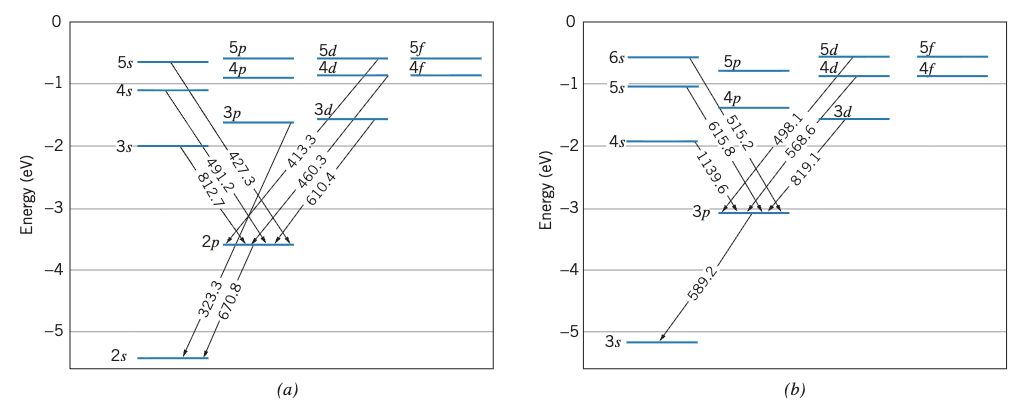
\includegraphics[width=\textwidth]{Images/Fig_8-4.png}
    \begin{center}
        Figure 8.4
    \end{center}
    \begin{enumerate}[label=(\alph*)]
        \item   Using the information for lithium given in Figure 8.4, compute the energy difference of the 3p and 3d states.
        \item   Compute the energy of the 3s, 4s, and 5s states above the ground state. 
        \item   The ionization energy of lithium in its ground state is 5.39 eV. 
                What is the ionization energy of the 2p state? 
                Of the 3s state?
    \end{enumerate}

    \subsection{Solution (a)}
        3p to 2s emits a photon of wavelength $\lambda = 323.3\,\unit{\nano\meter}$.
        3d to 2p emits a photon of wavelength $\lambda = 610.4\,\unit{\nano\meter}$.
        2p to 2s emits a photon of wavelength $\lambda = 670.8\,\unit{\nano\meter}$.
        From here, make a pathway from 3d to 3p, ensuring to make everything in terms of energy.
        \begin{align}
            E_{3d \to 3p}   &=  E_{3d \to 2p} + E_{2p \to 2s} - E_{3p \to 2s}
                =   hc\left( \frac{1}{\lambda_{3d \to 2p}} + \frac{1}{\lambda_{2p \to 2s}} - \frac{1}{\lambda_{3p \to 2s}} \right)\\
                &=  (1240\,\unit{\eV\cdot\nano\meter})\left( \frac{1}{610.4\,\unit{\nano\meter}} + \frac{1}{670.8\,\unit{\nano\meter}} - \frac{1}{323.3\,\unit{\nano\meter}} \right)\\
                &=  (1240\,\unit{\eV})\left( 1.64\E{-3} + 1.49\E{-3} - 3.09\E{-3} \right)\\
                &=  0.04 * 1240\,\unit{\eV}
                =   \boxed{49.6\,\unit{\eV}}
        \end{align}

    \subsection{Solution (b)}
        Assume 

\section{Problem 13} % 8.5
    Compute the $K_\alpha$ X ray energies of calcium (Z = 20), zirconium (Z = 40), and mercury (Z = 80). 
    Compare with the measured values of 3.69 keV, 15.8 keV, and 70.8 keV. 
    (See Question 16).

    \subsection{Solution}
        Calcium:
        $K_{\alpha}$ is the transition between $n = 2$ and $n = 1$.
        \begin{align}
            \Delta E    &=  (13.6\,\unit{\eV})(Z - 1)^2\left( \frac{1}{n_i^2} - \frac{1}{n_f^2} \right)
                =   (13.6\,\unit{\eV})19^2\left( \frac{1}{2^2} - \frac{1}{1^2} \right)
                =   \boxed{3.6822\,\unit{\kilo\eV}}
        \end{align}
        This is not far off from the measured value.
        
        Zirconium:
        \begin{align}
            \Delta E    &=  (13.6\,\unit{\eV})(Z - 1)^2\left( \frac{1}{n_i^2} - \frac{1}{n_f^2} \right)
                =   (13.6\,\unit{\eV})39^2\left( \frac{1}{2^2} - \frac{1}{1^2} \right)
                =   \boxed{15.5142\,\unit{\kilo\eV}}
        \end{align}
        This is not far off from the measured value.

        Mercury:
        \begin{align}
            \Delta E    &=  (13.6\,\unit{\eV})(Z - 1)^2\left( \frac{1}{n_i^2} - \frac{1}{n_f^2} \right)
                =   (13.6\,\unit{\eV})79^2\left( \frac{1}{2^2} - \frac{1}{1^2} \right)
                =   \boxed{63.6582\,\unit{\kilo\eV}}
        \end{align}
        This is much farther off from the measured value.
    \pagebreak

\section{Problem 15} % 8.6
    Use Hund's rules to find the ground-state L and S of (a) Ce, configuration [Xe]$6s^2 4f^1 5d^1$; (b) Gd, configuration [Xe]$6s^2 4f^7 5d^1$; (c) Pt, configuration [Xe]$6s^1 4f^{14} 5d^9$.

    \subsection{Solution (a)}
        Hund's rule says that $L = M_{L, max}$ and $S = M_{S, max}$.
        
        The electrons in the outermost shells are $4f^1 5d^1$.
        The maximum posible values for $m_l$ are $3$ for the $f$-orbital and $2$ for the $d$-orbital.
        Together, they total $L = M_{L, max} = 3 + 2 = \boxed{5}$.
        
        The electrons in the outermost shells are $4f^1 5d^1$.
        The maximum posible values for $m_s$ are $\frac{1}{2}$ both.
        Together, they total $S = M_{S, max} = \frac{1}{2} + \frac{1}{2} = \boxed{1}$.

    \subsection{Solution (b)}
        The electrons in the outermost shells are $4f^7 5d^1$.
        The maximum posible values for $m_l$ are two copies of 3, 2, and 1 and one copy of 0 from the $4f$ orbital, and one copy of 2 for the $d$-orbital.
        Together, they total $L = M_{L, max} = 2(3 + 2 + 1) + 2 + 0 = \boxed{14}$.
        
        The electrons in the outermost shells are $4f^1 5d^1$.
        At most, all 7 electrons in the $4f$ orbital would have value $\frac{1}{2}$, as with the one electron in the $5d$ orbital.
        Together, they total $S = M_{S, max} = 8 * \frac{1}{2} = \boxed{4}$.

    \subsection{Solution (c)}
        Here, the $4f$-orbital is full, so we can disregard that.
        In the $6s$ orbital, the maximum possible value of $m_l$ is just 0.
        In the $5d$ orbital, the maximum possible value of $M_L$ would come when only one value of $m_l$ is not taken up, being $-2$, which would make the total sum $L = \boxed{2}$.

        For a similar reason, the maximum possible value of $M_S$ is $S = \boxed{1}$.
    \pagebreak

\section{Problem 17}
    A certain excited state of an atom has the configuration $4d^1 5d^1$. 
    What are the possible L and S values?

\section{Problem 19} % 8.7
    A small helium-neon laser produces a light beam with an average power of 3.5 mW and a diameter of 2.4 mm.
    (a) How many photons per second are emitted by the laser?
    (b) What is the amplitude of the electric field of the light wave? 
    Compare this result with the electric field at a distance of 1 m from an incandescent light bulb that emits 100 W of visible light.

    \subsection{Solution (a)}
        A watt is equivalent to a joule per second.
        Since this is one second only, we can just multiply the power by one second to get the energy from one second to be $E = 3.5\,\unit{\milli\joule}$.
        Each HeNe laser photon has an energy of $1.96\,\unit{\eV}$, or $3.13\E{-19}\,\unit{\joule}$.
        Dividing the energy delivered by the energy of each photon, we get \boxed{1.11\E{16}} photons.
    
    \subsection{Solution (b)}
        First find the intensity.
        \begin{align}
            I   &=  \frac{P}{A} 
                =   \frac{3.5\,\unit{\milli\watt}}{\pi(1.2\,\unit{\milli\meter})^2}
                =   773.6\,\unit{\watt/\meter^2}\\
            E_0 &=  \sqrt{\frac{2I}{c\varepsilon_0}}
                =   \sqrt{\frac{2 * 773.6\,\unit{\watt/\meter^2}}{2.998\E{8}\,\unit{\meter/\second} * 8.85\E{-12}\,\unit{\coulomb^2/(\newton\meter^2)}}}\\
                &=  \sqrt{\frac{1547.2}{2.65\E{-3}}}\,\unit{\newton/\coulomb}
                =   \sqrt{583900}\,\unit{\newton/\coulomb}
                =   \boxed{764\,\unit{\newton/\coulomb}}
        \end{align}
\end{document}